\section{Lecture 5 | Model Free Control}

\subsubsection*{Off and On Policy Learning}
\begin{itemize}
  \item On Policy Learning - Learn about policy \(\pi \) from experience sampled from \(\pi \).
  \item Off Policy Learning - Learn about policy \(\pi \) from experience sampled from \(\mu \).
\end{itemize}

\subsection{On Pilocy Monte Carlo Control}

\begin{figure}[H]
    \begin{minipage}{0.5\textwidth}
        \begin{itemize}
            \item Policy Evaluation - Estimate \(v_\pi \) e.g. Iterative Policy Evaluation. 
            \item Policy Improvement - Generate \(\pi' \geq \pi \) e.g. Greedy Policy Improvement.
          \end{itemize}
    \end{minipage}%
    \begin{minipage}{0.5\textwidth}
      % Your image goes here
      \centering
      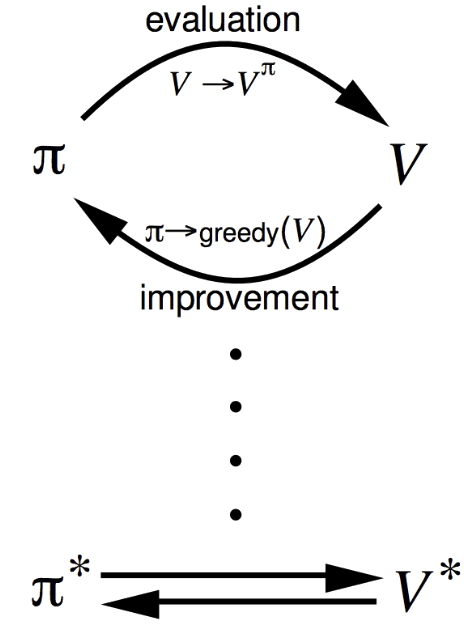
\includegraphics[height=0.75\textwidth]{figures/gpi.png}
      \caption{Generalised Policy Iteration}
        \label{fig:gpi}
    \end{minipage}
  \end{figure}

One of the simple ideas is to use Monte Carlo Policy Evaluation and Greedy Policy Improvement.
BUt this quickly runs into problems:
\begin{itemize}
  \item Policy Evaluation - Monte Carlo Policy Evaluation with value function, requires
  the model of the MDP.
  \item Policy Improvement - Greedy Policy Improvement faces the issue of the
  expectation of the entire state space.
\end{itemize}
So, greefy policy improvemnent over \(V(s)\) requires model of the MDP.
\[
  \pi'(s) = \argmax_{a \in \mathcal{A}(s)} \mathcal{R}^a_s + \mathcal{P} ^a_{ss'} V(s')
\]
replacing the value function with stae action value function, the policy evaluation is model
free.
\[
  \pi'(s) = \argmax_{a \in \mathcal{A}(s)} Q(s,a)
\]

\subsubsection{\(\epsilon\)-Greedy Exploration}
This is one of the simplest ways to explore the state space. The idea is to choose the greedy
action with probability \(1-\epsilon\) and a random action with probability \(\epsilon\). 
Thus all \(m\) actions have a non-zero probability of being selected. 
\[
  \pi(a|s) = \begin{cases}
    1-\epsilon + \frac{\epsilon}{m} & \text{if } a^{\star}  = \argmax\limits_
    {a \in \mathcal{A}(s)} Q(s,a) \\
    \frac{\epsilon}{m} & \text{otherwise}
  \end{cases}
\]


\begin{theorem}[\(\epsilon \)-Greedy Policy Improvement]
  For any \(\epsilon \)-greedy policy \(\pi\), the \(\epsilon \)-greedy policy \(\pi'\) with
  respect to \(q_\pi \) is an improvement, \(v_{\pi'}(s) \geq v_\pi(s)\).
\end{theorem}
\begin{proof}
  \begin{align*}
    q_\pi(s, \pi'(s)) &= \sum_{a \in \mathcal{A}(s)} \pi'(a|s) q_\pi(s,a) \\
    &= \frac{\epsilon}{m} \sum_{a \in \mathcal{A}(s)} q_\pi(s,a) + (1-\epsilon) \max_{a \in
    \mathcal{A}(s)} q_\pi(s,a) \\
    &\geq \frac{\epsilon}{m} \sum_{a \in \mathcal{A}(s)} q_\pi(s,a) + (1-\epsilon) \sum_{a
    \in \mathcal{A}(s)} \frac{\pi(a|s) - \frac{\epsilon}{m}}{1-\epsilon} q_\pi(s,a) \\
    &= \sum_{a \in \mathcal{A}(s)} \pi(a|s) q_\pi(s,a) = v_\pi(s)
  \end{align*}
  Therefore from policy improvement theorem, \(v_{\pi'}(s) \geq v_\pi(s)\).
\end{proof} 

Thus the Monte Carlo Control can be summarissed as follows:
\begin{figure}[H]
  \begin{minipage}{0.5\textwidth}
    Every episode:
      \begin{itemize}
          \item Policy Evaluation - Monte Carlo Policy Evaluation with value function : 
          \(Q \approx q_\pi \) 
          \item Policy Improvement - \(\epsilon \)-Greedy Policy Improvement.
        \end{itemize}
  \end{minipage}%
  \begin{minipage}{0.5\textwidth}
    % Your image goes here
    \centering
    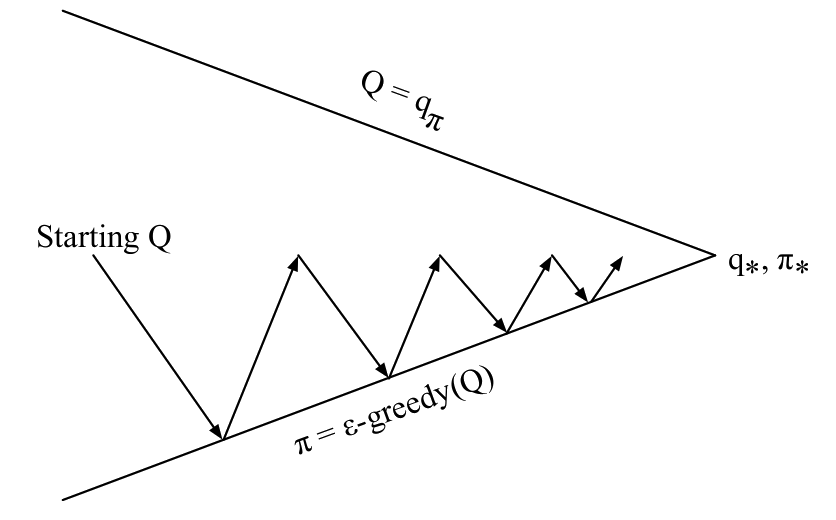
\includegraphics[width=\textwidth]{figures/mc-eps.png}
    \caption{Monte Carlo Control}
    \label{fig:mc-eps}
  \end{minipage}
\end{figure}

\subsubsection{GLIE}
GLIE = Greedy in the Limit with Infinite Exploration.

\begin{theorem}[Greedy in the Limit with Infinite Exploration]
  If all state-action pairs are explored infinitely many times, then the policy converges
  to a greedy policy, \(\lim_{k \to \infty} \pi_k(a|s) = \mathbb{1}(a = \argmax_{a \in
  \mathcal{A}(s)} Q(s,a))\).
  Thus, GLIE has these two properties:
  \begin{itemize}
    \item Every state-action pair is visited infinitely many times.
    \[
      \lim_{k \to \infty} N_k(s,a) = \infty
    \]
    \item The policy converges on a greedy policy.
    \[
      \lim_{k \to \infty} \pi_k(a|s) = \bm{1}(a = \argmax_{a \in \mathcal{A}(s)} Q(s,a))
    \]
  \end{itemize}
\end{theorem}
For example, \(\epsilon\)-greedy with \(\epsilon = \frac{1}{k}\) for the \(k^{th}\) episode
satisfies GLIE.

\subsubsection{GLIE Monte Carlo Control}
The algortihm can be described as:
\begin{itemize}
  \item Sample \(k^{th}\) episode using \(\pi_k\): \(S_0, A_0, R_1, \dots, S_{T}\)
  \item For each state \(S_t\) and action \(A_t\) in the episode:
  \[
    \begin{aligned}
      N(S_t, A_t) &\leftarrow N(S_t, A_t) + 1 \\
      Q(S_t, A_t) &\leftarrow Q(S_t, A_t) + \frac{1}{N(S_t, A_t)} (G_t - Q(S_t, A_t)) \\
      \pi(S_t) &\leftarrow \argmax_{a \in \mathcal{A}(S_t)} Q(S_t, a)  
    \end{aligned}
  \]
  \item Improve the policy based on new action value function.
  \[
    \begin{aligned}
      \epsilon &\leftarrow \frac{1}{k} \\
      \pi &\leftarrow \epsilon\text{-greedy}(Q)
    \end{aligned}
  \]
\end{itemize}
\begin{theorem}[Convergence of GLIE Monte Carlo Control]
  GLIE Monte Carlo Control converges to the optimal action-value function, \(Q(s,a) \to
  q_\star(s,a)\).
\end{theorem}

\subsection{SARSA(\(\lambda \))}
Use the natureal idea to replace MC wtth TD(\(\lambda\)). So we will be applying,
TD to the action value function, \(Q(s,a)\), by using the \(\epsilon\)-greedy policy
improvement. The policy is updated at every time step.

Thus at every time step:
\begin{itemize}
  \item Policy Evaluation - SARSA(\(\lambda\)) : \(Q \approx q_\pi \)
  \[
    Q(S,A) \leftarrow Q(S,A) + \alpha \left( 
      R + \gamma Q(S', A') - Q(S,A)
     \right) 
  \]
  \item Policy Improvement - \(\epsilon\)-Greedy Policy Improvement.
\end{itemize}
The algorithm for SARSA is shown in \autoref{alg:sarsa}.
\begin{algorithm}[H]
  \caption{SARSA}
  \label{alg:sarsa}
  \begin{algorithmic}[1]
    \State Initialise \(Q(s,a)\) arbitrarily and \(E(s,a) = 0\) for all \(s \in \mathcal{S},
    a \in \mathcal{A}(s)\)
    \State Q(terminal-state, \(\cdot\)) = 0
    \For{each episode}
      \State Initialise \(S\)
      \State Choose \(A\) from \(S\) using policy derived from \(Q\) (e.g.
      \(\epsilon\)-greedy)
      \For{each step of episode}
        \State Take action \(A\), observe \(R, S'\)
        \State Choose \(A'\) from \(S'\) using policy derived from \(Q\) (e.g.
        \(\epsilon\)-greedy)
        \State \(Q(s,a) \leftarrow Q(s,a) + \alpha \left[ 
          R + \gamma Q(S', A') - Q(S,A)
         \right] \)
        \State \(S \leftarrow S'\), \(A \leftarrow A'\)
      \EndFor
    \EndFor
  \end{algorithmic}
\end{algorithm}

\begin{theorem}[Convergence of SARSA]
  SARSA converges to the optimal action-value function, \(Q(s,a) \to q_\star(s,a)\), under
  the following conditions:
  \begin{itemize}
    \item GLIE sequence of policies \(p_t(a|s)\) 
    \item Robbins-Monro sequence of step-sizes
    \[
      \begin{aligned}
        \sum_{t=1}^{\infty} \alpha_t(s,a) &= \infty \\
        \sum_{t=1}^{\infty} \alpha_t^2(s,a) &< \infty
      \end{aligned}
    \]
    The first equation ensures that the steps are large enough to overcome the initial
    conditions and the second equation ensures that the steps are small enough to converge.

  \end{itemize}
\end{theorem}
